% Set the author and title of the compiled pdf
\hypersetup{
  pdftitle = {\Title},
  pdfauthor = {\Author}
}

In Semester One, of this course we covered zero and non-zero sum games (Nash
games) and search algorithms to find equlibriums (minimax and alpha beta
pruning). In this semester, we are no longer assuming that each player has the
same `role' and the games are zero-sum. We are letting there be an infinite
number of positions for each player and not assuming perfect information.

We're going to be looking at Stackelberg games; an example of which could be
retail pricing. Different firms might offer different prices on products, they
can choose infinite price points (or close enough) and some firms might have
private information that others might not.

An industry can be controlled or dominated by a one, more or entity:

\begin{description}
  \item \textbf{Monopoly}: When an industry consists of a single firm.
  \item \textbf{Duopoly}: When an industry consists of two firms.
  \item \textbf{Oligopoly}: When an industry consists of a few firms (and when
  each decision one takes impacts on the other's profits).
\end{description}

In duopoly/oligopoly situations, the roles of the players are different. If one
firm chooses to change its prices first, then the others have to decide what to
do in light of the change; and may not know the full economic and/or political
motivations behind the initial move.

In a two player Stackelberg game, one player selects his strategy first, and
then the other responds. The first player is called the leader ($P_L$) and the
second is called the follower ($P_F$). In a Nash game, the players select their
strategy simultaneously.

There are payoff functions for the leader and follower, where each player wants
to maximise their own:

\[
  J_L(U_L, U_F)
\]

\[
  J_F(U_L, U_F)
\]

A strategy space is the set of all possible strategies for a single player. The
leader's strategy space is $U_L$ and the follower's is $U_F$. They can include
finite (discrete) or infinite (continuous) strategies. The leader must choose
$u_L \in U_L$ and the follower must choose $u_F \in U_F$.

% Slide 20??

In a Stackelberg game, the leader first announces his strategy $u_L$, and then
the follower selects his best response $R(uL) \in U_F$ which maximises:

\[
  J_F(u_L, R(u_L)) = MAX_{u_F \in U_F} J_F(u_L, u_F)
\]

In order to solve a Stackelberg game, we need to solve the following problem:

\begin{itemize}
  \item What is the follower's reaction function $R(u_L)$?
  \item When we've found that, what leader strategy $u_L$ maximises the leader's
  payoff function:
  \[
    J_L(u^*_L, R(u^*_L)) = MAX_{u_L \in U_L} J_L(u_L, u_L)
  \]
\end{itemize}

If the follower has a reaction function $R(U_L)$ and there exists a leader
strategy $U^*_L \in U_L$ and the response strategy is $u^*_F = R(U^*_L) \in U_F$
such that $J_L(u^*_L, u^*_F) = MAX_{u_L \in U_L} J_L(u_L, R(u_L))$, then
$(u^*_L, u^*_F)$ is called a \textbf{Stackelberg strategy/equilibrium}.

We always assume that the follower is rational and tries to find the best
reaction strategy. Sometimes this is untrue, for example if taking a non-optimal
strategy results in a rival player having a big loss.

For a player to be a leader, he needs to act first. There is no requirement that
they are a leader in an economic or political sense. The only requirement to be
a follower is to act second; the follower is not necessarily in a weaker
position. As mentioned before, Stackelberg games can be continuous or discrete,
depending on if the strategy space is finite or infinite.

Since the only difference between a Nash game and a Stackelberg game is whether
moves are played simultaneously or in order, should we prefer Nash or
Stackelberg games? If the player has the opportunity to be the leader, then
Stackelberg games should be preferred, since he will always be better off than in
a Nash game in this instance. Here's a mini-proof:

Let $u_1$ and $u_2$ be the strategies for player's one and two, and let
$J_1(u_1, u_2)$, $J_2(u_1, u_2)$ be their respective payoff functions. If there
is a Stackelberg strategy and a Nash strategy, then:

\[
  J_1(u^{Stackelberg}_1, u^{Stackelberg}_2) \geq J_1(u^{Nash}_1, u^{Nash}_2)
\]

I don't understand the next bit on page 29...

% TODO: Understand proof on P29

Note that sometimes the follower can be better off in a Stackelberg game, but
the leader would still be better off playing the Stackelberg game than playing a
Nash game. Other times, the player could win as the leader or follower, but win
better as the follower.

For the follower to play the game, he needs to know nothing about the leader or
his strategy space. However, for the leader to play, he needs to know the
follower's payoff function and strategy space in order to work out the action
that will give the max payoff. If such information is not available, then the
leader must guess or learn it (based off previous experience or data).

% Lecture 2

\section{Solving Stackelberg game problems}

We can solve with two sequential maximisation problems, each for a single
player:

\begin{enumerate}
  \item For each of the leader's strategies $u_L \in U_L$, solve:
    \[
      max_{u_F \in U_F}(J_F(u_L, u_F)
    \]
    The solution for this is the follower's reaction function $R(u_L)$.
  \item Find the best strategy for the leader by solving:
    \[
      max_{u_L \in U_L}(J_L[u_L, R(u_L)])
    \]
    If $u^*_L$ is the strategy found in the above maximisation, and
    $u^*_L = R(u^*_L)$, then ($u^*_L, u^*_F)$ is a Stackelberg strategy.
\end{enumerate}

So, in order to find the Stackelberg strategy, we need to solve two maximisation
problems. This is A-level maths, but we can recap it in the next bit.

\subsection{How to find the maximum point of a function over a continuous space}

We want to find a point $x^* \in X$ that maximises $f(x)$ over $X$, such that
$\forall x \in X, f(x^*) \geq f(x)$. Such a point is called the global maximum
point of $f(x)$ on $X$. A local maximum point $y^*$ is the maximum value of
$f(x)$ within the region $U$, such that $\forall x \in U, f(y^*) \geq f(x)$.

\begin{figure}
  \centering
  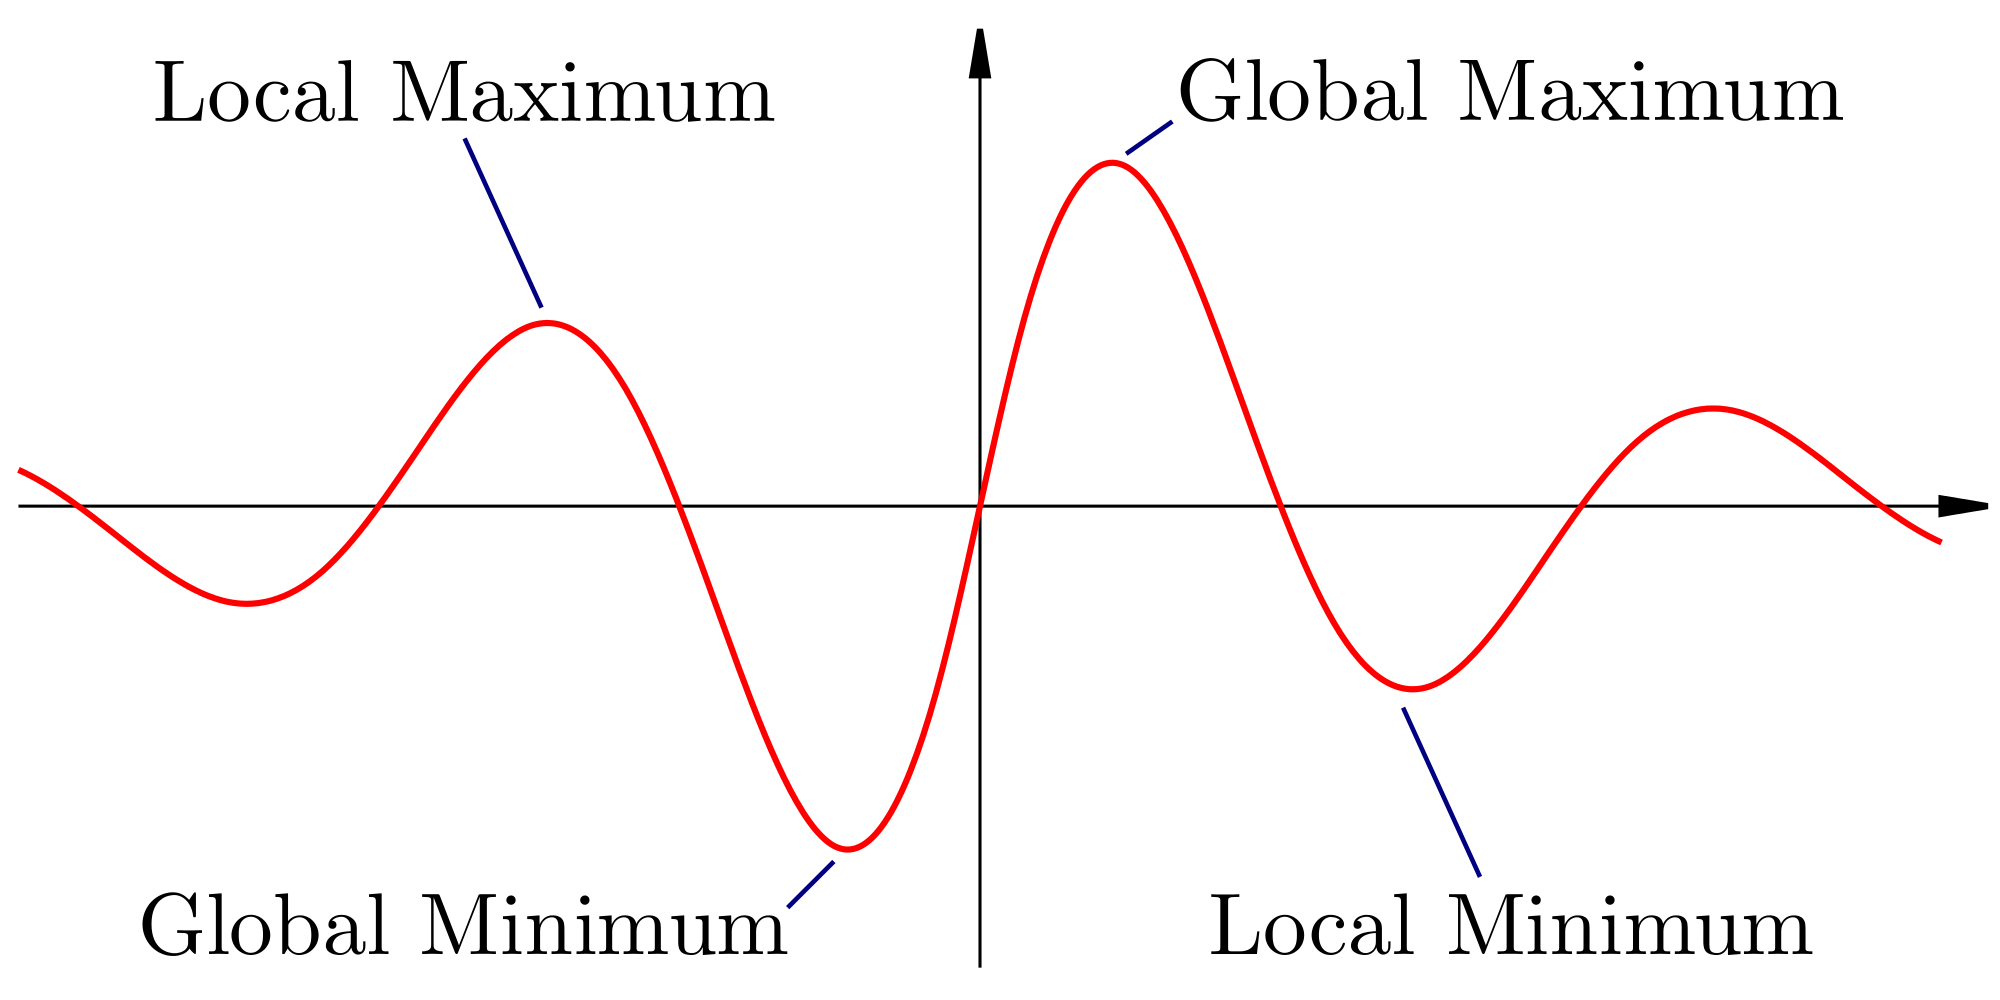
\includegraphics[width=\textwidth]{images/maxima}
  \caption{Wikipedia's pictorial explanation of minima and maxima.}
  \label{fig:maxima}
\end{figure}

The standard method for trying to find a maximum of a function is by using
derivatives. A derivative is usually notated by a dash after the function.
Finding the derivative of a derivative is called the second order derivative
function, and has two dashes.

A first order derivative represents the gradient of the line drawn by the
function at a specific point. If $f'(x) > 0$, then the line slopes upwards, and
if $f'(x) < 0$ then it's sloping down. Obviously if it is equal to zero, then
the line is horizontal.

%TODO: Is this finding derivitives linear time?

\subsubsection{Calculating a derivative}

The most simple rule is: 

\[
  f(x) = x^n \therefore f'(x) = nx^{n-1}
\]

This means if the function is constant, it disappears:

\[
  f(x) = C \therefore f'(x) = 0
\]

Here are three simple examples:

\[
  f(x) = x^2 \therefore f'(x) = 2x
\]

\[
  f(x) = x^3 \therefore f'(x) = 3x^2
\]

If a function is composed of other functions that are added together (of the form $f(x) = f_1(x) + \dots + f_n(x)$ then:

\[
  f'(x) = f_1'(x) + \dots + f_n'(x)
\]

Just like:

\[
  f(x) = -2x^2 + 4x + 5 \therefore f'(x) = -4x + 4
\]

Finally, if it's composed of functions that are multiplied together, then
$f'(x)= f_1'(x)f_2(x) + f_1(x)f_2'(x)$:

\[
  f(x) = x^2 \times x \therefore
    f'(x) = [x^2]' \times x + x^2 \times [x]' = 2x \times x + x^2 \times 1
          = 2x^2 + x^2 = 3x^2
\]

\subsubsection{Finding maxima}

Once you've found the derivative of your function, and then found the points
where the derivatives are 0 (and the gradient of the line is therefore zero),
you need to determine whether that point is a minima or maxima. To do this, we
differentiate again to get the second order derivative. If the value of $f''(x)
\geq 0$ then the gradient is increasing, therefore it's a minima. Because of
this, we want points where the second order derivative gives a negative value,
indicating that the point is a maxima.

To find the largest maxima, we simply find the one that is largest value of
$f(x)$.

% See slide 15